\documentclass[11pt]{article}

\usepackage[a4paper,margin=1in]{geometry}
\usepackage{amsmath,amssymb}
\usepackage{booktabs}
\usepackage{graphicx}
\usepackage{float}
\usepackage{hyperref}
\usepackage{xcolor}

\title{Paper I: Finite-Horizon Value Analysis for a Simple Markov Reward Process}
\author{}
\date{\today}

\begin{document}
\maketitle

\begin{abstract}
This note summarizes a first set of finite-horizon Markov Reward Process (MRP) experiments for a four-state example with transition-level rewards. For a grid of discount factors $\gamma \in \{0, 0.05, \dots, 1\}$, we compute exact finite-horizon state values by Bellman recursion and compare them against Monte Carlo estimates with confidence intervals. We report two main runs, both using $100$ trajectories per state and discount factor, with horizons $H=20$ and $H=50$. The exact ranking of states is stable across the full grid and both horizons: \texttt{Computer} $>$ \texttt{Coffee} $>$ \texttt{Home} $>$ \texttt{Chat}.
\end{abstract}

\section{The MRP}
The state space is
\[
S = \{\texttt{Chat}, \texttt{Coffee}, \texttt{Computer}, \texttt{Home}\}.
\]

The transition probabilities and rewards are:

\begin{center}
\begin{tabular}{llll}
\toprule
From & To & Probability & Reward \\
\midrule
\texttt{Chat} & \texttt{Chat} & 0.5 & -1 \\
\texttt{Chat} & \texttt{Coffee} & 0.2 & 1 \\
\texttt{Chat} & \texttt{Computer} & 0.3 & 2 \\
\texttt{Coffee} & \texttt{Chat} & 0.7 & 2 \\
\texttt{Coffee} & \texttt{Coffee} & 0.1 & 1 \\
\texttt{Coffee} & \texttt{Computer} & 0.2 & 3 \\
\texttt{Computer} & \texttt{Chat} & 0.1 & -3 \\
\texttt{Computer} & \texttt{Coffee} & 0.2 & 1 \\
\texttt{Computer} & \texttt{Computer} & 0.5 & 5 \\
\texttt{Computer} & \texttt{Home} & 0.2 & 2 \\
\texttt{Home} & \texttt{Coffee} & 0.4 & 1 \\
\texttt{Home} & \texttt{Home} & 0.6 & 1 \\
\bottomrule
\end{tabular}
\end{center}

Figure~\ref{fig:mrp-graph} shows the visualization used in this project.

\begin{figure}[H]
\centering
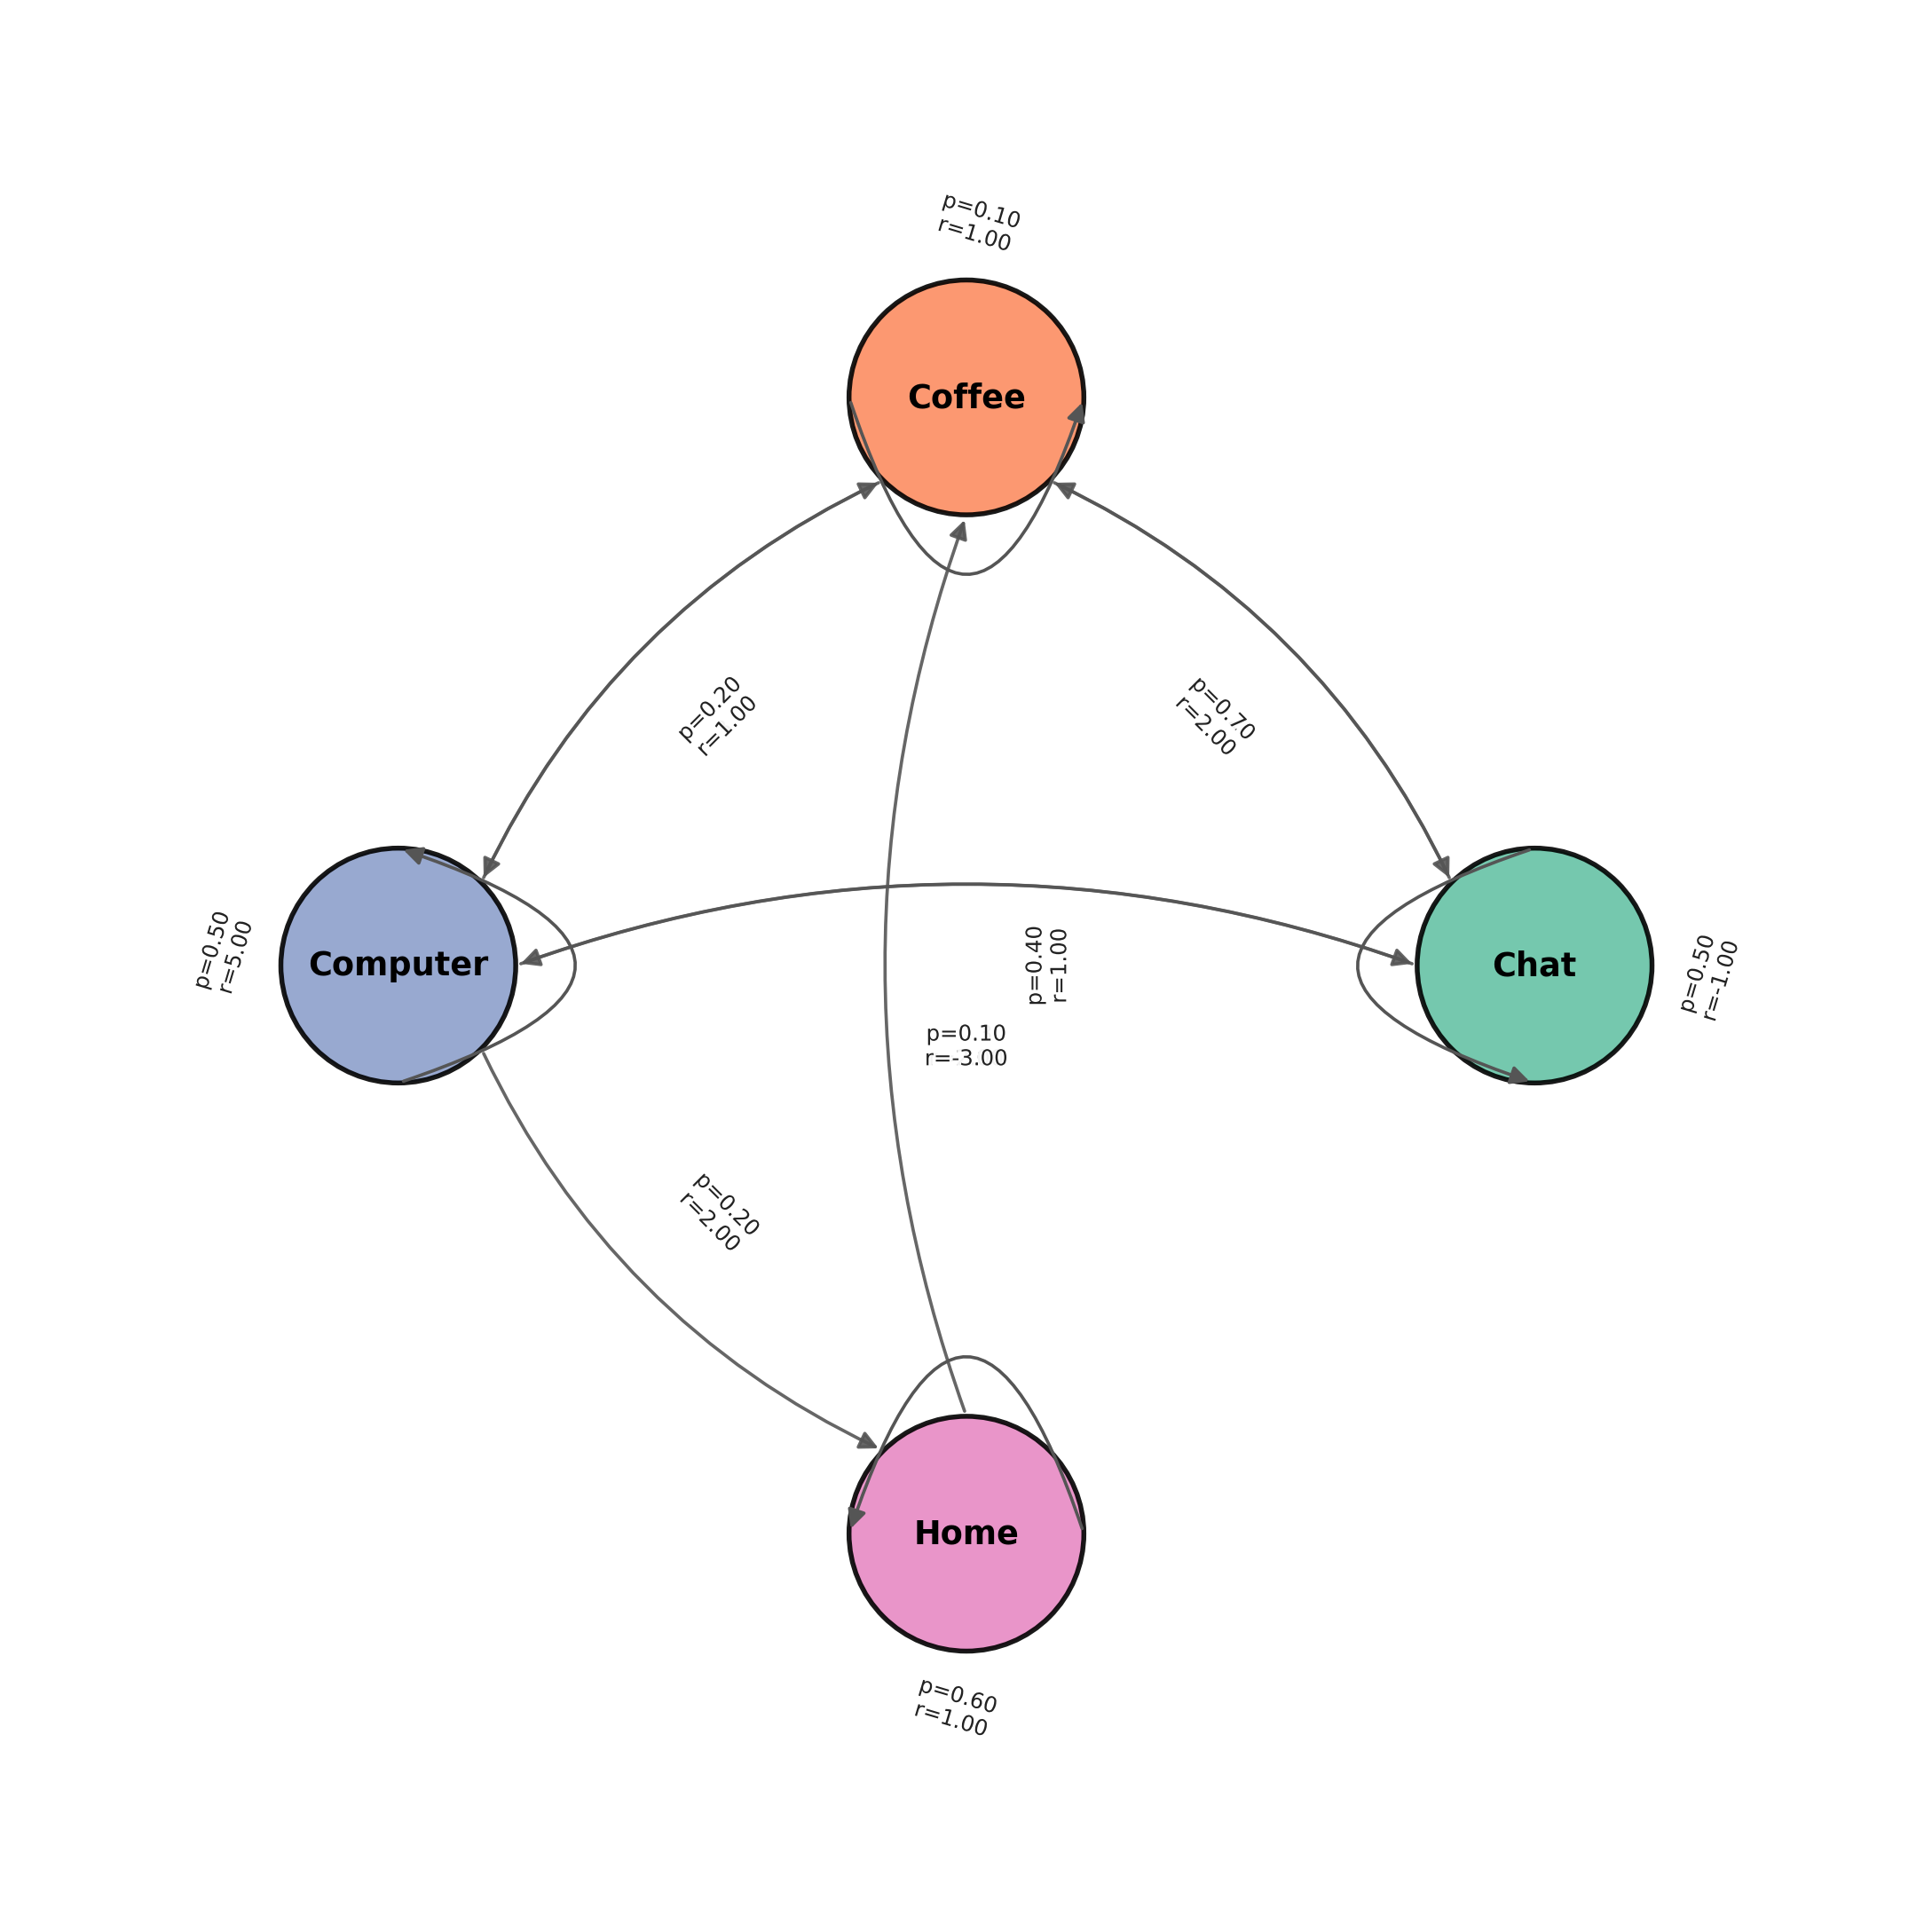
\includegraphics[width=0.78\textwidth]{figures/simple_mrp_visualization.png}
\caption{The four-state Markov Reward Process. Edge labels show transition probability $p$ and immediate reward $r$.}
\label{fig:mrp-graph}
\end{figure}

\section{Exact Finite-Horizon Values}
For a horizon $H$, define the finite-horizon return
\[
G_0^{(H)} = r_1 + \gamma r_2 + \cdots + \gamma^{H-1} r_H.
\]
The exact finite-horizon value function is
\[
V_H(s) = \mathbb{E}[G_0^{(H)} \mid s_0 = s].
\]

Because rewards are attached to transitions, the Bellman recursion is
\[
V_0(s) = 0,
\]
\[
V_H(s) = \sum_{s'} P(s' \mid s)\left(R(s,s') + \gamma V_{H-1}(s')\right).
\]

This recursion is exact and cheap for the present MRP, so it serves as the reference quantity for all comparisons against Monte Carlo estimates.

\section{Experimental Protocol}
For each $\gamma \in \{0, 0.05, \dots, 1\}$ and each start state, we ran:
\begin{itemize}
  \item exact finite-horizon evaluation by Bellman recursion;
  \item Monte Carlo estimation from $100$ trajectories;
  \item a $95\%$ confidence interval for the Monte Carlo mean.
\end{itemize}

Two main result directories were used:
\begin{itemize}
  \item \texttt{MRP/outputs\_100traj\_th10}, whose CSV files actually record \textbf{$H=20$};
  \item \texttt{MRP/outputs\_100traj\_th50}, with \textbf{$H=50$}.
\end{itemize}

The directory name \texttt{th10} is therefore misleading; the paper uses the actual horizon value stored in the output files.

\section{Main Results}

\subsection{State ranking}
Across the full $\gamma$ grid and both horizons, the exact ordering never changes:
\[
\texttt{Computer} > \texttt{Coffee} > \texttt{Home} > \texttt{Chat}.
\]

This is already visible at $\gamma=0$, where values reduce to expected one-step rewards, and it remains true up to $\gamma=1$ under the chosen finite horizons.

\subsection{Representative exact values}
Table~\ref{tab:representative-values} lists exact values at three representative discount factors.

\begin{table}[H]
\centering
\begin{tabular}{llrrrr}
\toprule
Horizon & $\gamma$ & \texttt{Computer} & \texttt{Coffee} & \texttt{Home} & \texttt{Chat} \\
\midrule
20 & 0.00 & 2.8000 & 2.1000 & 1.0000 & 0.3000 \\
20 & 0.50 & 4.6158 & 3.3484 & 2.3852 & 1.7696 \\
20 & 1.00 & 32.1830 & 30.3916 & 29.1096 & 29.0409 \\
\midrule
50 & 0.00 & 2.8000 & 2.1000 & 1.0000 & 0.3000 \\
50 & 0.50 & 4.6158 & 3.3484 & 2.3852 & 1.7696 \\
50 & 1.00 & 77.5669 & 75.7755 & 74.4935 & 74.4248 \\
\bottomrule
\end{tabular}
\caption{Representative exact finite-horizon values. Increasing the horizon has no visible effect at $\gamma=0$, little effect at moderate discounting, and a large effect when $\gamma=1$.}
\label{tab:representative-values}
\end{table}

\subsection{Monte Carlo accuracy}
Table~\ref{tab:error-summary} summarizes absolute errors between the Monte Carlo estimates and exact values over the full state-discount grid.

\begin{table}[H]
\centering
\begin{tabular}{lrrr}
\toprule
Horizon & Mean absolute error & Maximum absolute error & Worst-$\gamma$ mean error \\
\midrule
20 & 0.3016 & 2.4670 & $\gamma=1.00$: 1.7840 \\
50 & 0.2500 & 2.3252 & $\gamma=1.00$: 1.1398 \\
\bottomrule
\end{tabular}
\caption{Aggregate Monte Carlo error summary using $100$ trajectories per state and discount factor. The hardest regime is $\gamma=1$, where long-horizon variance is highest.}
\label{tab:error-summary}
\end{table}

The finite-horizon Monte Carlo estimates are generally close to the exact values for small and moderate $\gamma$, but the error grows substantially near $\gamma=1$. This is expected: as discounting weakens, later rewards matter more, and finite-sample variance becomes larger.

\section{Figures}

\begin{figure}[H]
\centering
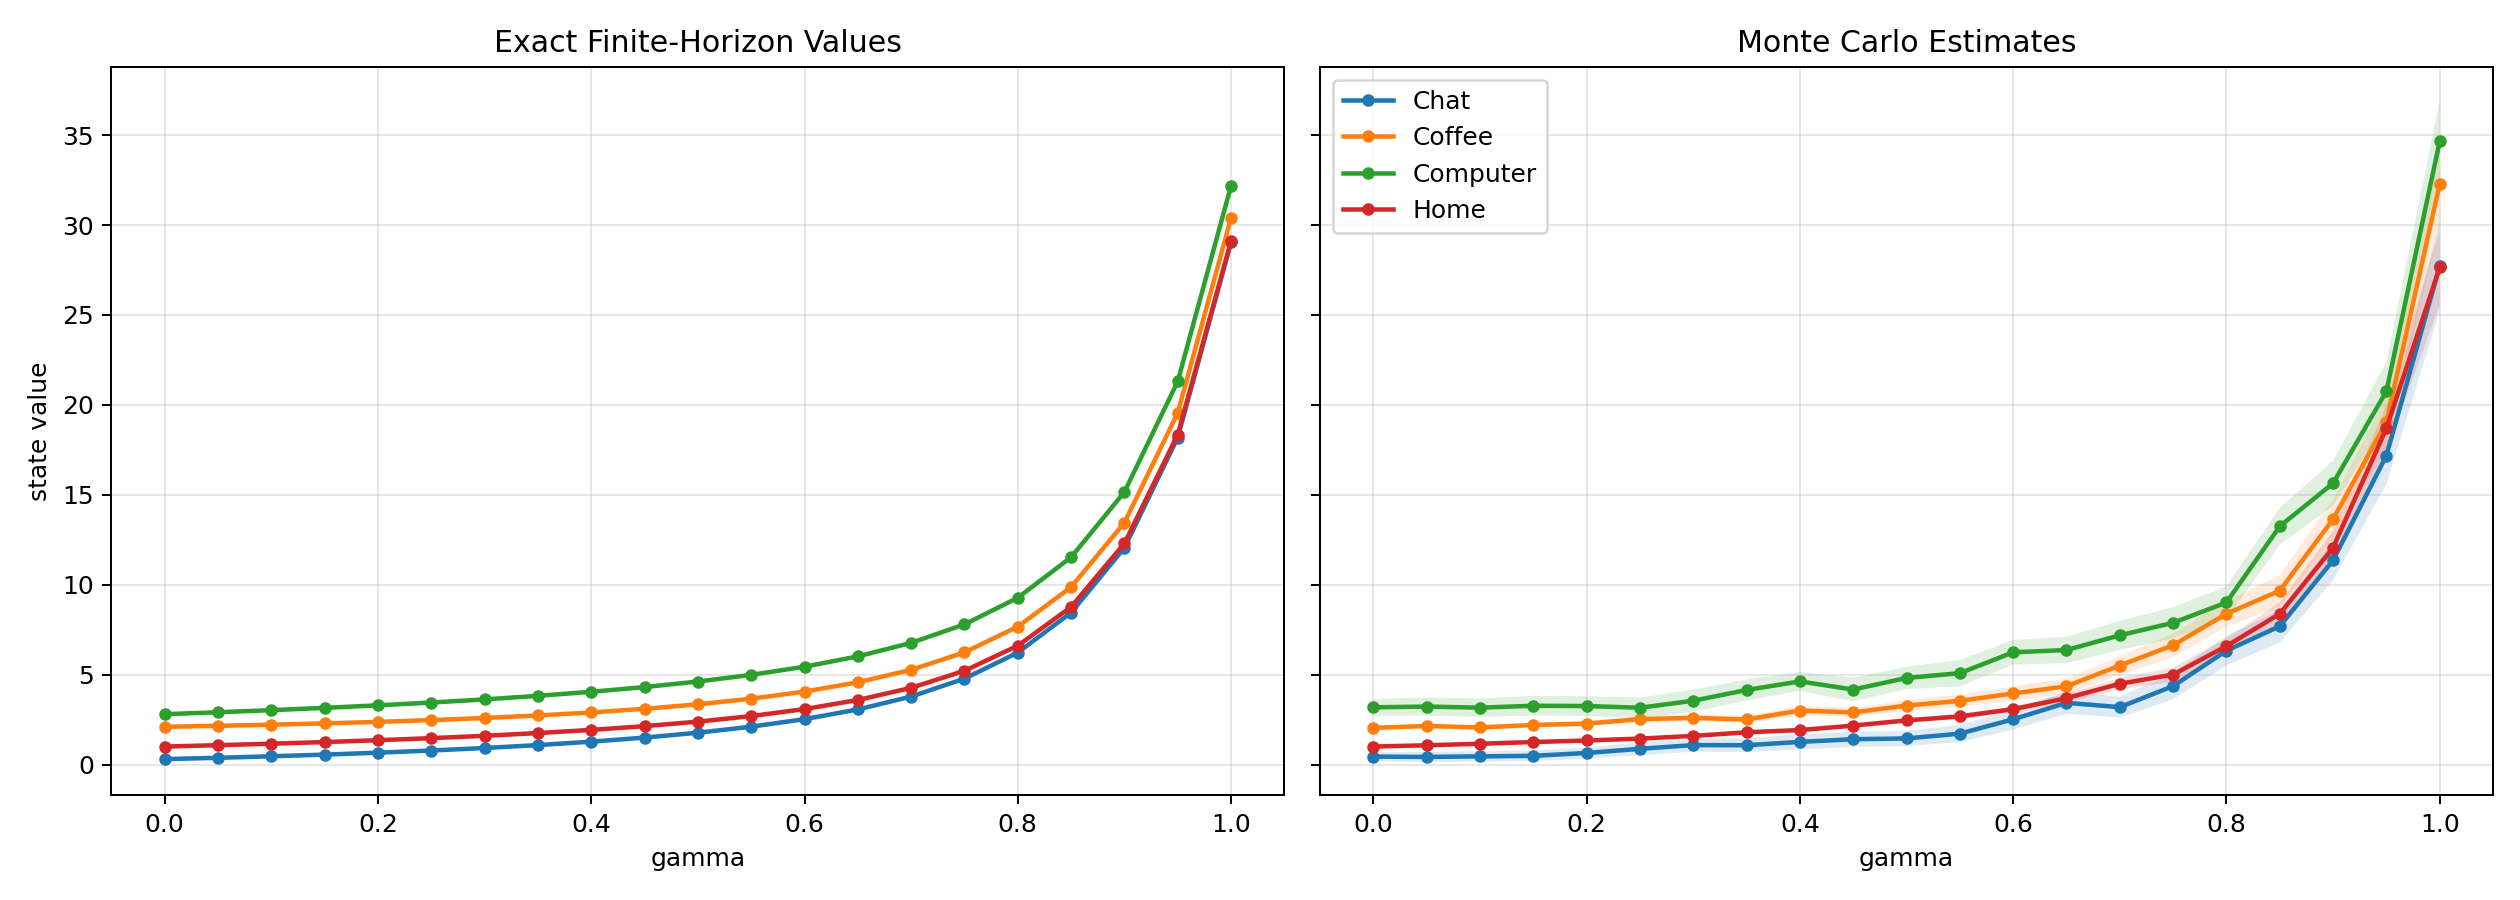
\includegraphics[width=0.95\textwidth]{figures/value_vs_gamma_th10.png}
\caption{Exact values and Monte Carlo estimates with $95\%$ confidence bands for the run stored in \texttt{outputs\_100traj\_th10}. The CSV metadata show that this corresponds to horizon $H=20$.}
\label{fig:values-h20}
\end{figure}

\begin{figure}[H]
\centering
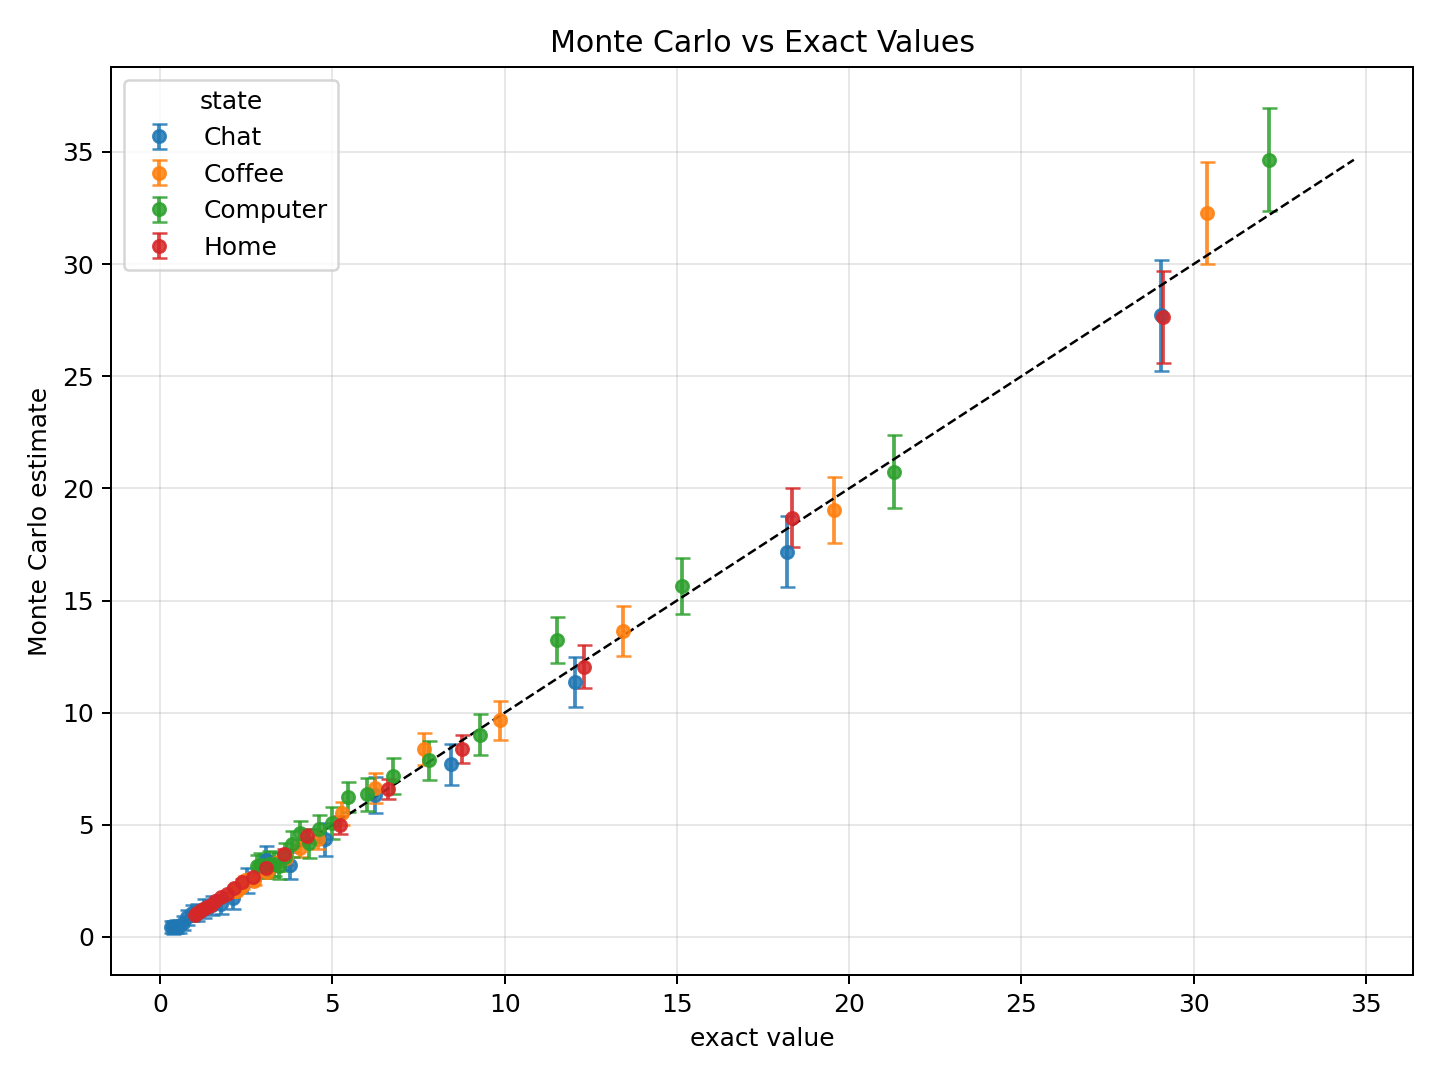
\includegraphics[width=0.72\textwidth]{figures/comparison_exact_vs_mc_th10.png}
\caption{Exact vs Monte Carlo estimates for the $H=20$ run. The diagonal line is the identity reference.}
\label{fig:scatter-h20}
\end{figure}

\begin{figure}[H]
\centering
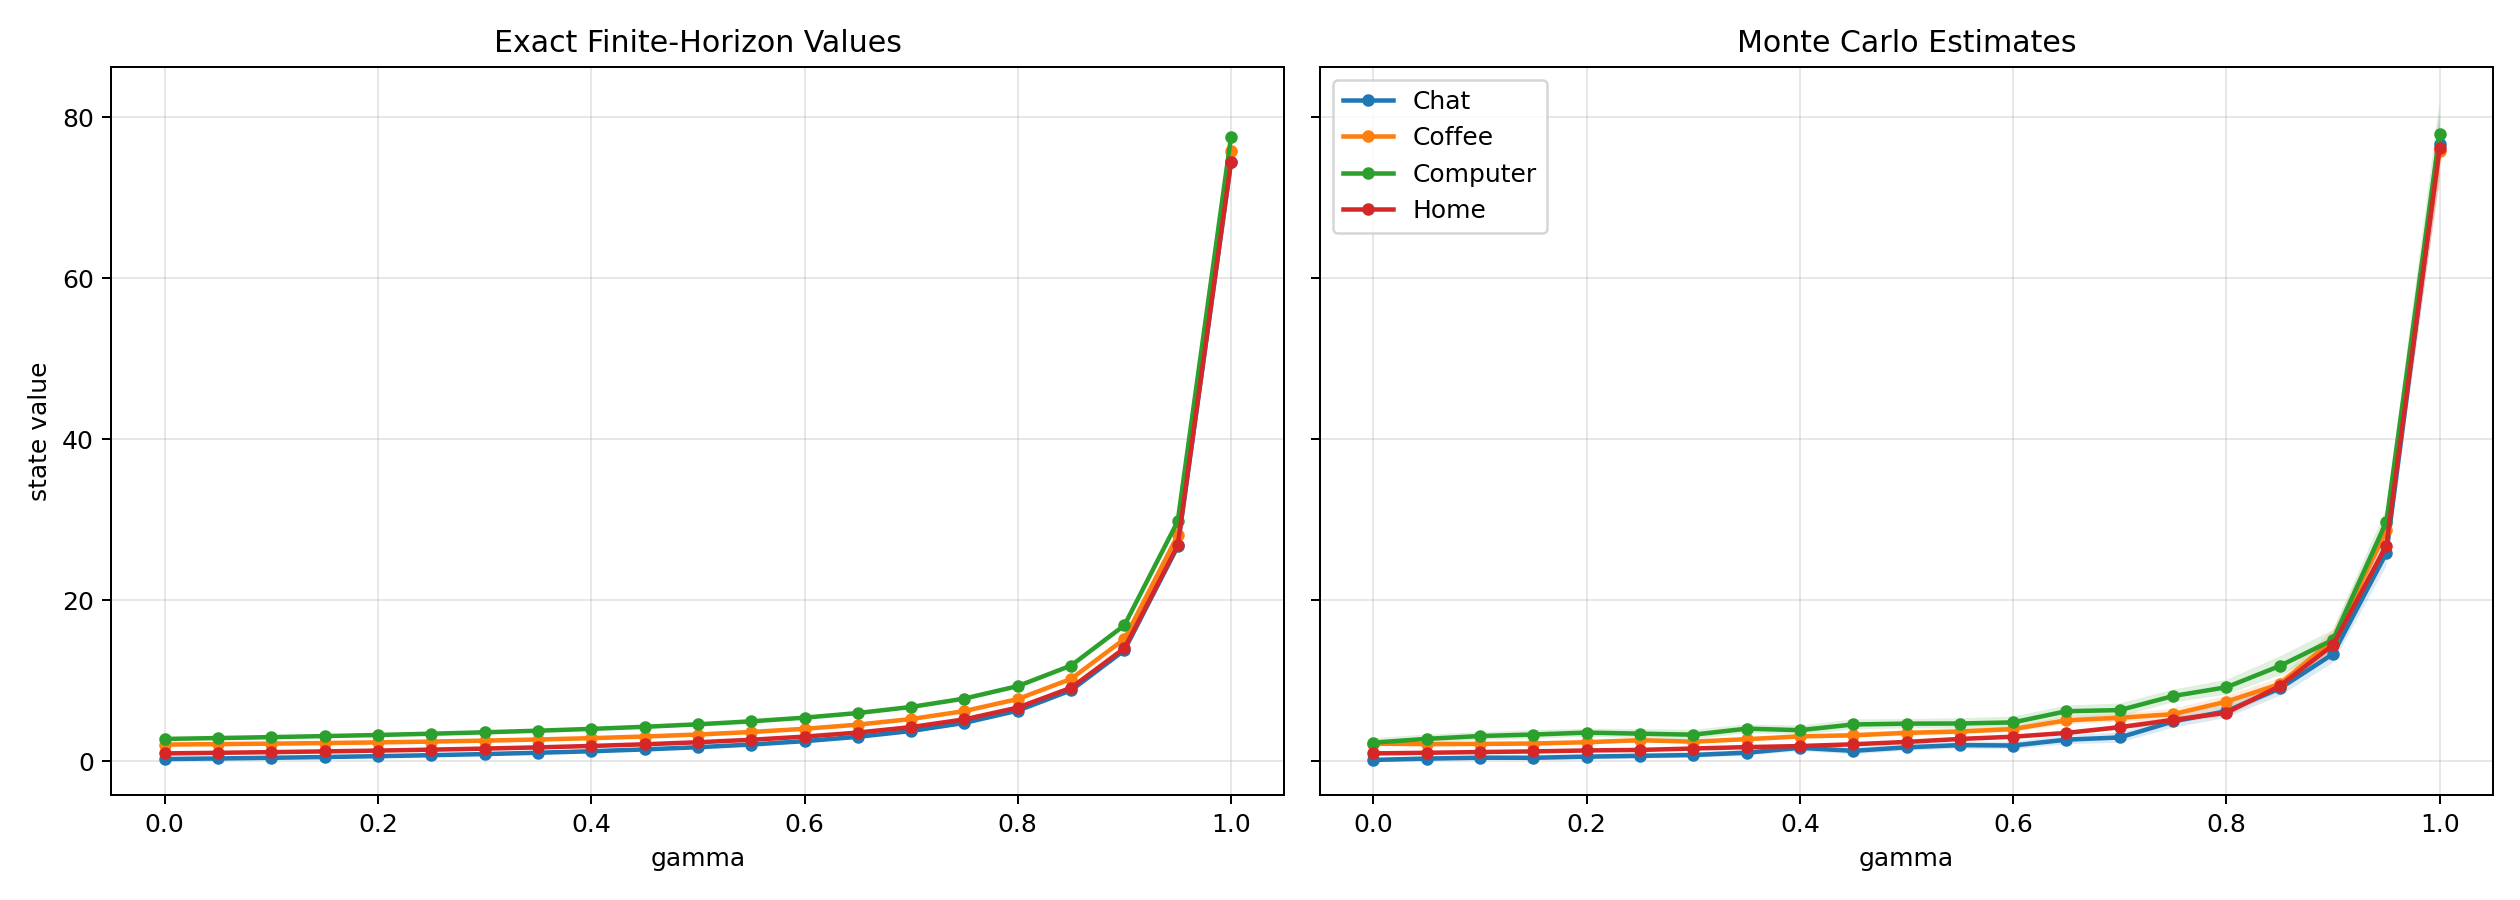
\includegraphics[width=0.95\textwidth]{figures/value_vs_gamma_th50.png}
\caption{Exact values and Monte Carlo estimates with $95\%$ confidence bands for horizon $H=50$.}
\label{fig:values-h50}
\end{figure}

\begin{figure}[H]
\centering
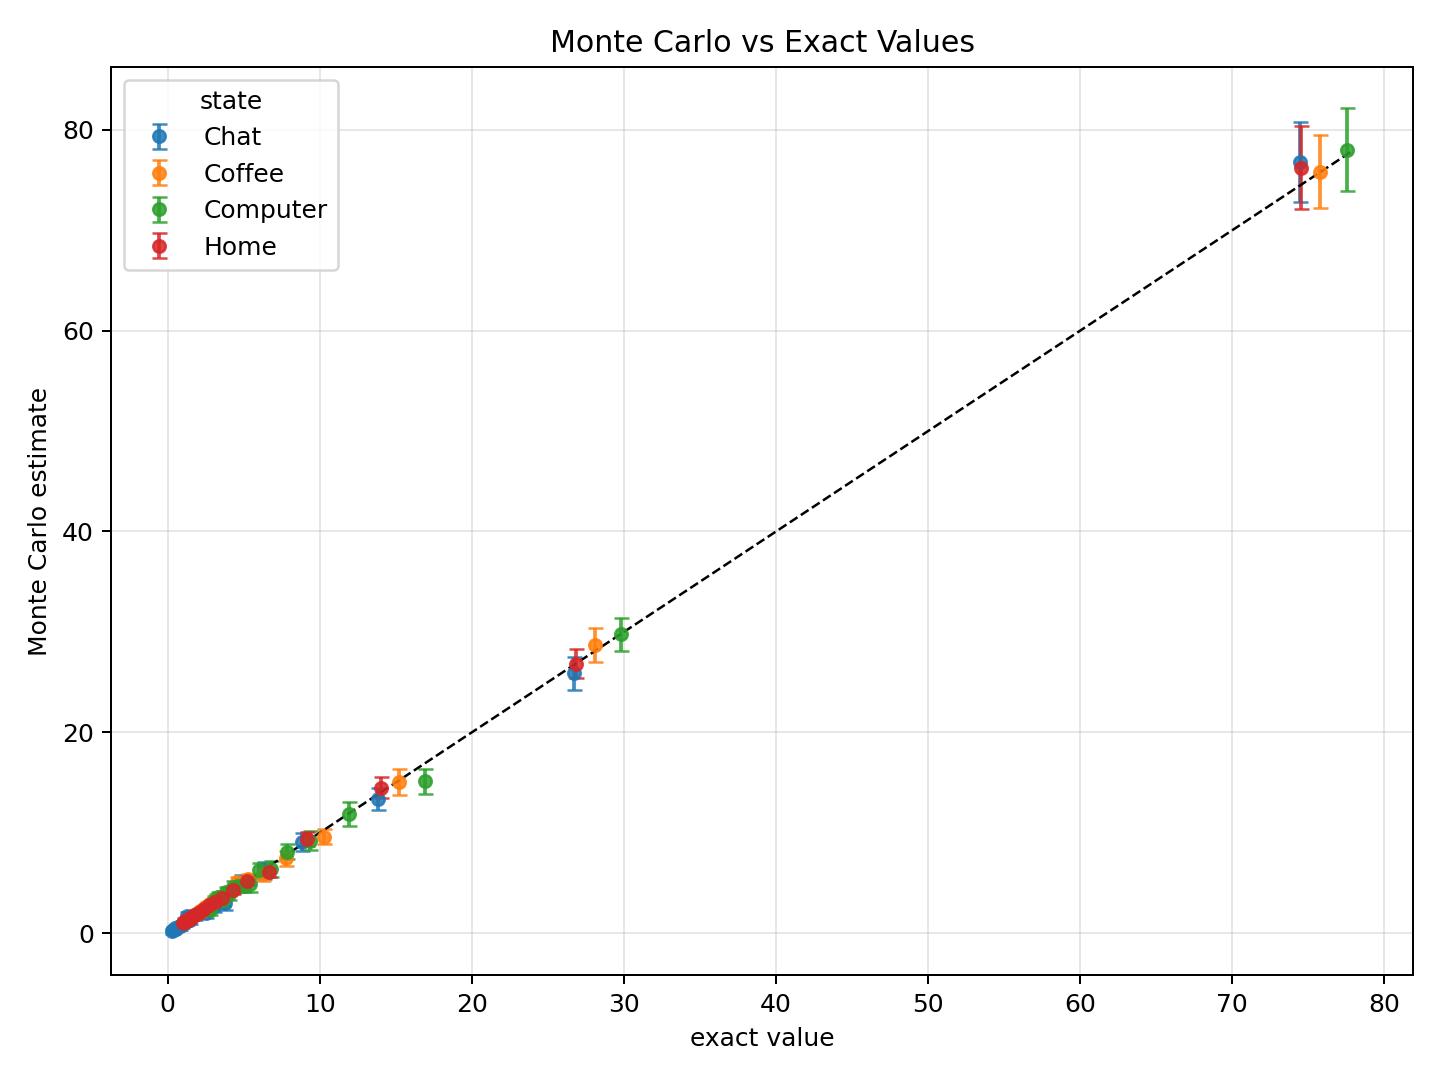
\includegraphics[width=0.72\textwidth]{figures/comparison_exact_vs_mc_th50.png}
\caption{Exact vs Monte Carlo estimates for the $H=50$ run.}
\label{fig:scatter-h50}
\end{figure}

\section{Interpretation}
Three simple points stand out.
\begin{enumerate}
  \item \textbf{The ranking is robust.} \texttt{Computer} is always the highest-value start state, followed by \texttt{Coffee}, then \texttt{Home}, then \texttt{Chat}.
  \item \textbf{Horizon matters most when $\gamma$ is large.} At $\gamma=0.5$, the exact values for $H=20$ and $H=50$ are effectively identical at the reported precision. At $\gamma=1$, the longer horizon produces much larger values.
  \item \textbf{Monte Carlo variance is the limiting factor near $\gamma=1$.} Even with $100$ trajectories, the difficult region is the weak-discount regime, where the cumulative reward has higher variance.
\end{enumerate}

\section{Conclusion}
This first paper establishes a clean baseline for the project: the simple MRP is fully specified, exact finite-horizon values are available by Bellman recursion, Monte Carlo estimates can be checked against ground truth, and the main qualitative ranking is stable across horizons and discount factors. The most natural next extensions are infinite-horizon analysis for $\gamma < 1$, trajectory-count sensitivity, and ensemble experiments on randomly generated MRPs.

\end{document}
